\begin{frame}
    \frametitle{Проблема проверки алгоритма на данных с известным оптимумом}
    \begin{figure}
        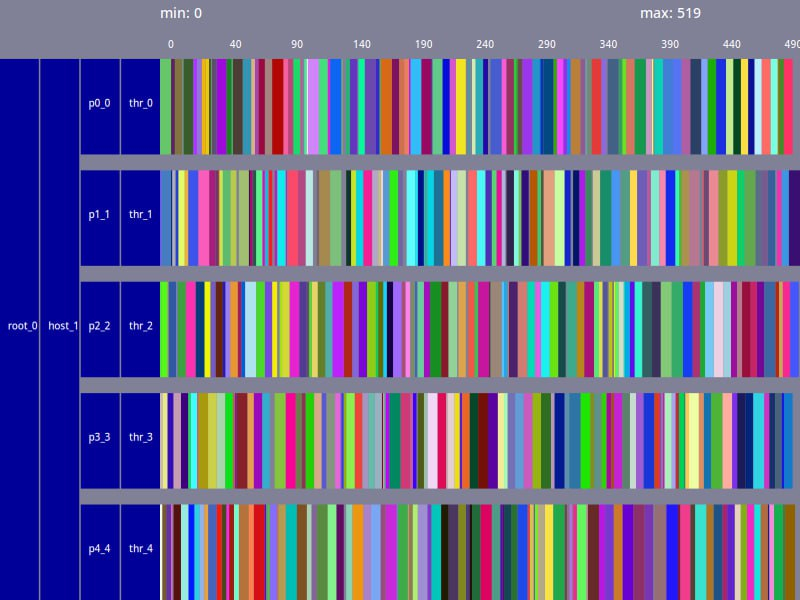
\includegraphics[width=0.6\textwidth]{imgs/balanced-schedule.jpg}
    \end{figure}
\end{frame}

\begin{frame}
    \frametitle{Точность полученного расписания. CR и NO}
    \begin{figure}
        \begin{subfigure}{0.49\textwidth}
            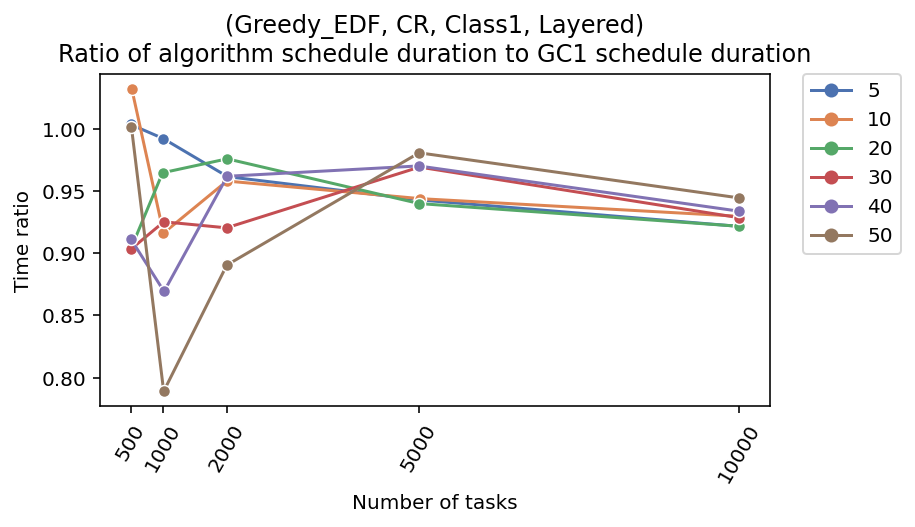
\includegraphics[width=\textwidth]{imgs/layered_class_1/CR_EDF/gr_amalgamated.png}
            \caption{При постановке CR}
        \end{subfigure}
        \begin{subfigure}{0.49\textwidth}
            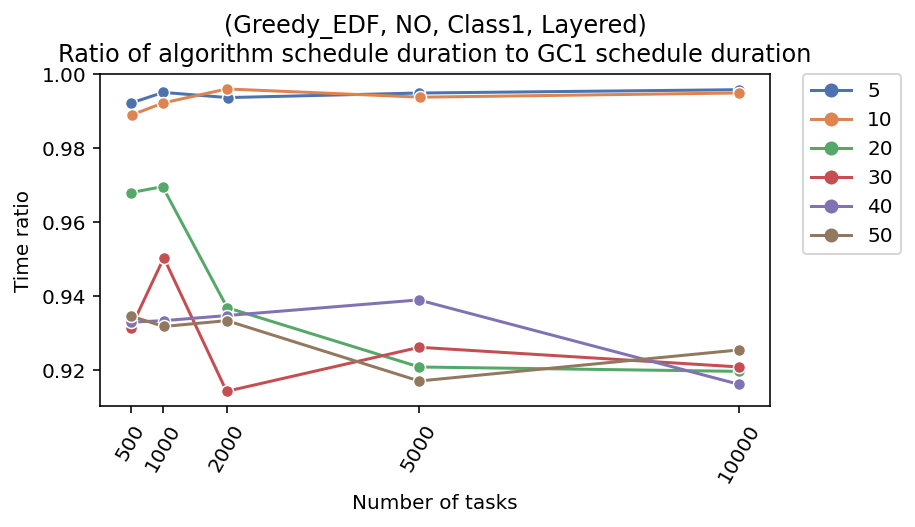
\includegraphics[width=\textwidth]{imgs/layered_class_1/NO_EDF/gr_amalgamated.png}
            \caption{При постановке NO}
        \end{subfigure}
        \caption{Отношение длительности работы алгоритма с фиктивными директивными сроками к длительности\\работы жадного алгоритма на данных, основанных на слоистых графах}
    \end{figure}
\end{frame}

\begin{frame}
    \frametitle{Точность полученного расписания. CR и NO}
    \begin{figure}
        \begin{subfigure}{0.49\textwidth}
            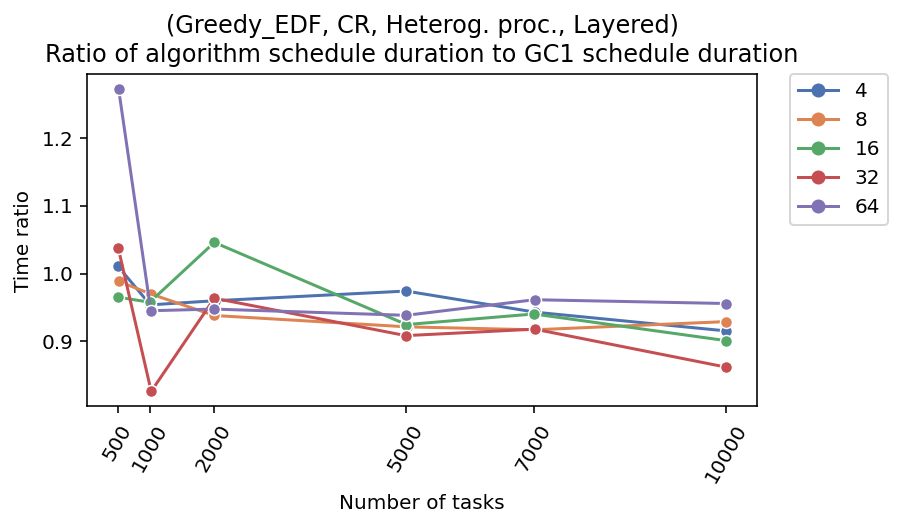
\includegraphics[width=\textwidth]{imgs/unbalanced/CR_EDF/gr_amalgamated.png}
            \caption{При постановке CR}
        \end{subfigure}
        \begin{subfigure}{0.49\textwidth}
            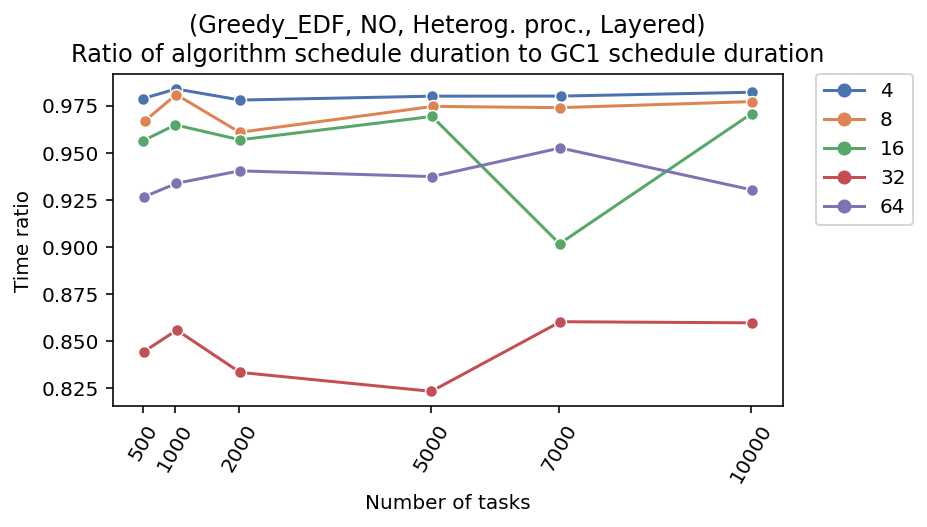
\includegraphics[width=\textwidth]{imgs/unbalanced/NO_EDF/gr_amalgamated.png}
            \caption{При постановке NO}
        \end{subfigure}
        \caption{Отношение длительности работы алгоритма с фиктивными директивными сроками к длительности\\работы жадного алгоритма на данных, основанных на неоднородных процессорах}
    \end{figure}
\end{frame}

\begin{frame}
    \frametitle{Время выполнения программы. CR и NO.}
    \begin{figure}
        \begin{subfigure}{0.49\textwidth}
            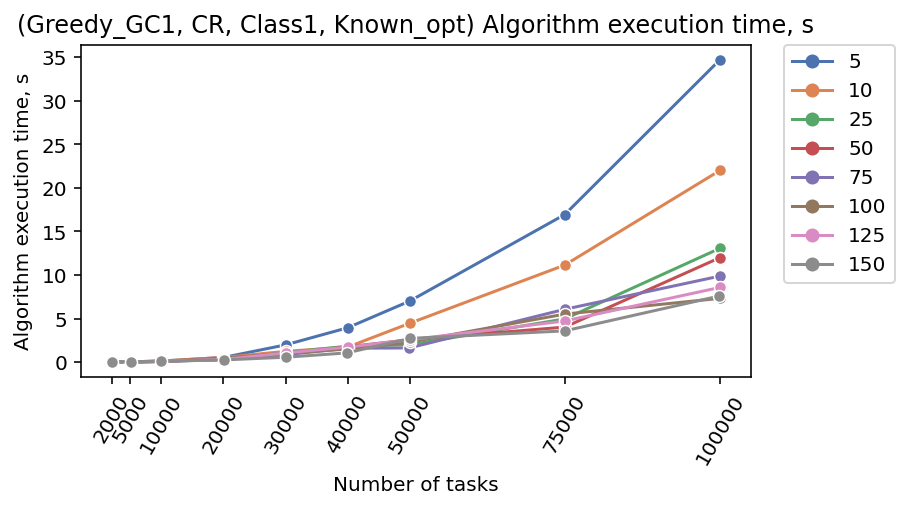
\includegraphics[width=\textwidth]{imgs/ideal_1/CR/tr_graph.png}
            \caption{Жадный алгоритм с выбором по числу потомков}
        \end{subfigure}
        \begin{subfigure}{0.49\textwidth}
            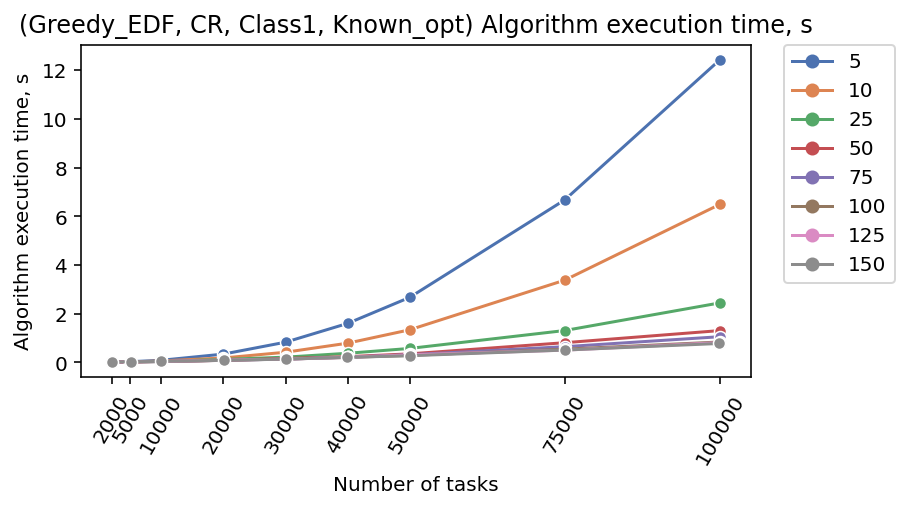
\includegraphics[width=\textwidth]{imgs/ideal_1/CR_EDF/tr_graph.png}
            \caption{Жадный алгоритм с фиктивными директивными сроками}
        \end{subfigure}
        \caption{Время выполнения алгоритма на данных с известным оптимумом, в секундах}
    \end{figure}
\end{frame}
